\begin{figure}[t]
\centering
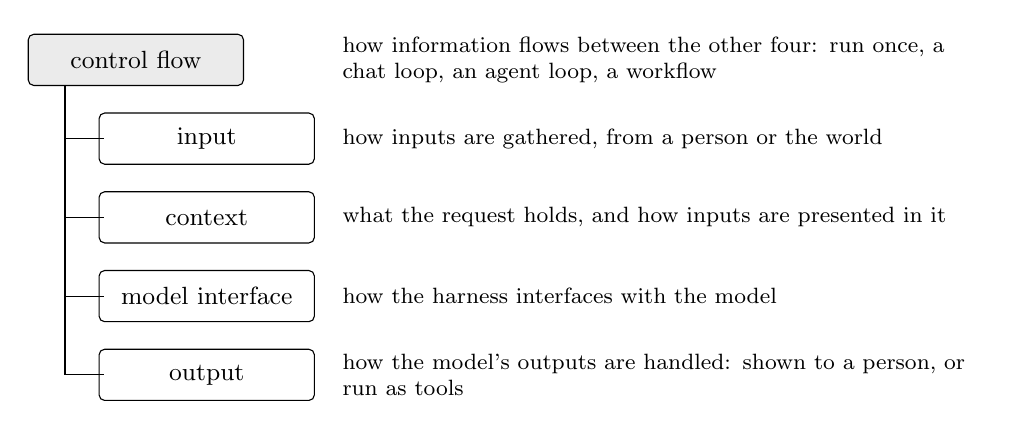
\begin{tikzpicture}[
  box/.style={draw, rounded corners=2pt, minimum height=6.5mm, text width=25mm, align=center, font=\small},
  note/.style={font=\footnotesize, text width=80mm, align=left, anchor=west}]
\node[box, fill=black!8] (cf) at (0,0) {control flow};
\node[note] at (2.5,0) {how information flows between the other four: run once, a chat loop, an agent loop, a workflow};
\foreach \y/\name/\txt in {-1/input/{how inputs are gathered, from a person or the world},
                           -2/context/{what the request holds, and how inputs are presented in it},
                           -3/model interface/{how the harness interfaces with the model},
                           -4/output/{how the model's outputs are handled: shown to a person, or run as tools}} {
  \node[box] at (0.9,\y) {\name};
  \node[note] at (2.5,\y) {\txt};
  \draw (-0.9,\y) -- (-0.4,\y);
}
\draw (-0.9,-0.33) -- (-0.9,-4);
\end{tikzpicture}
\caption{The five primitives of a harness. Control flow wraps the other four.}
\label{fig:tree}
\end{figure}
